\subsection{Основные определения. Теорема о ранге и дефекте линейных отображений}

\deff{def:} $U,V$ - линейное пространства над одним полем $K(\mathbb{R}, \mathbb{C})$.

$\mathcal{A}: U\rightarrow V$ называется \deff{линейным гомоморфизмом}, если: 
$$\forall \lambda \in K,\forall u_1, u_2 \in U: \mathcal{A}(u_1 + \lambda u_2) = \mathcal{A} (u_1) + \lambda\mathcal{A}(u_2)$$

\textbf{Замечание 1:} Мы будем писать $\mathcal{A} u$, вместо $\mathcal{A}(u)$.

\textbf{Замечание 2:} $\mathcal{A}u, \mathcal{B}u$ это какие-то числа, поэтому мы можем складывать их и умножать на скаляр.

\textbf{Замечание 3:} $\mathcal{A} \zero_U = \zero_V$, частный случай $\lambda = 0$

\textbf{Примеры:}
\begin{enumerate}
    \item $\zero$: это нулевое отображения $\forall u \in U: \zero u = 0$ 

    \item $P_n$ - пространство многочленов степени $\leq n$. $\mathcal{A}=\cfrac{d}{dx}$ --- дифферинцирование.

    \item $\varepsilon$ --- тождественное отображение. $\varepsilon: U\rightarrow U:\forall u\in U: \varepsilon u = u$.
\end{enumerate}


\deff{Введем операции:}
\begin{enumerate}
    \item $\lambda \in K: \mathcal{A}$ --- линейное отображение. Введем операцию умножения:
$$\ \forall u \in U: (\lambda\mathcal{A}) u = \lambda(\mathcal{A} u)$$
    \item $\mathcal{A}, \mathcal{B}$ --- линейные отображение. Введем операцию cложения: 
    $$ \forall u \in U:(\mathcal{A} + \mathcal{B}) u = \mathcal{A}u + \mathcal{B}u $$
    

    \item  $\mathcal{B}\in L(U,W)$, $\mathcal{A} \in (L(W,V)$. Введем операцию произведения:
    $$\forall u \in U:(\mathcal{A} \cdot \mathcal{B}) u = \mathcal{A}(\mathcal{B}u)$$
    
\end{enumerate}


 $\Im \mathcal{A} = \{v \in V:v =\mathcal{A} u| \forall u\in U \}$ --- \deff{образ линейного пространства.}

\textbf{Замечание:} $\Im \mathcal{A}$ --- линейное подпространство.

$\ker  \mathcal{A} = \{u \in U| \mathcal{A} u = \zero\}$ %
--- \deff{ядро линейного отображения}.

 $\rg \mathcal{A} = \dim \Im \mathcal{A}$ --- \deff{ранг отображения} 

 $def \mathcal{A} = \dim \ker \mathcal{A}$ --- \deff{дефект отображения.}

\newpage

\textbf{Виды отображений:}

\begin{itemize}
    \item сюръекция, если $\Im \mathcal{A} = V \Leftrightarrow \rg \mathcal{A}= \dim V$.
    \item инъекция, если $\ker A = \{\zero_U\} \Leftrightarrow def A = 0$.

    \item биекция или изоморфизм $\Leftrightarrow \begin{cases}
        \Im \mathcal{A} = V\\
        \ker \mathcal{A} = \{\zero_U\}
    \end{cases} \Leftrightarrow \begin{cases}
        \rg \mathcal{A} = \dim V \\
        def \mathcal{A} = 0
    \end{cases}$
    \item \emph{эндоморфизмом} или линейным оператором, когда $U = V$.

    $\mathcal{A} \in End(V) = End_K(v)$ %
    \item \emph{автоморфизм} это биекция + эндоморфизм.
    
     $\mathcal{A} \in Aut(V) = Aut_K(v)$ %
\end{itemize}

\textbf{Примеры:}

\begin{enumerate}
    \item $P_n$ --- пространство многочленов степени не больше n. $\mathcal{A}= \cfrac{d}{dt} $ $\mathcal{A}:P_n \rightarrow P_n$. не инъекция, не сюръекция, не изоморофизм, эндоморфизм и не автоморфизм
    \item $U = K^n, V = K^m$, $A = (a_{ij})_{m\times n}, a_{ij} \in K$,  $\forall u \in U   :\mathcal{A}u=A\cdot u$.

    $\Im \mathcal{A} = \left\{y\in K^m \begin{array}{cc}
         y = \mathcal{A}x \\
          \forall x \in K^n
    \end{array}\right\} = \span (A_1,\ldots,A_n)$ --- \emph{образ матрицы}.

    $y = A\cdot x = \sum\limits_{i=1}^nA_i\cdot x_i$

    Давайте более подробно рассмотрим \emph{отображения}:

    \begin{itemize}
        \item[1.] сюръекция $\Leftrightarrow \rg \mathcal{A} = \dim V  = m$.

        $\ker \mathcal{A} = \{x \in K^n: Ax = \zero\}$ --- общее решение СЛОУ, 
        \emph{ядро матрицы}.

        $\dim \ker \mathcal{A} = \dim $ общего решения $= n - \rg A$.

            $def \mathcal{A} = n - rg A$ --- \emph{дефект матрицы.}

        \item[2.] инъекция $\Leftrightarrow def A=0 \Leftrightarrow n-\rg A = 0 \Leftrightarrow \rg A = n$.

        \item[3.] биекция $\Leftrightarrow \begin{cases}
            \rg A = n \\
            \rg A = m
        \end{cases} \Leftrightarrow n = m$.

        \item[4.] эндоморфизм $\Leftrightarrow n = m \Leftrightarrow A_{n \times n}$.

        \item[5.] автоморфизм $\Leftrightarrow rg \mathcal{A} = n, A_{n\times n }\Leftrightarrow \exists A^{-1}$.
    \end{itemize}
    
   
\end{enumerate}


\textbf{Свойства произведения:}
\begin{enumerate}
    \item $\mathcal{A}, \mathcal{B}$ --- изоморф. $\Rightarrow \mathcal{A} \cdot \mathcal{B}$ --- изоморфно.
    \item $\mathcal{A}(\mathcal{B}_1 + \mathcal{B}_2) =  \mathcal{A} \mathcal{B}_1 + \mathcal{A} \mathcal{B}_2$.
    \item  $\forall \lambda \in K: \mathcal{A}(\lambda \mathcal{B}) = (\lambda \mathcal{A}) \mathcal{B} = \lambda (\mathcal{A} \cdot \mathcal{B})$.
    \item $\mathcal{C} \in L(\Omega, U): \mathcal{A} \cdot (\mathcal{B}\cdot \mathcal{C}) = (\mathcal{A}\cdot \mathcal{B}) \cdot \mathcal{C}$
\end{enumerate}

Ассоциативная унитальная алгебра.

    \textbf{Замечание 1.} Если $\mathcal{A} \in L(U,V)$ --- изоморфно $\Rightarrow \mathcal{A}^{-1}$ --- взаимно обр. отображение.

\textbf{Замечание 2.} Если $\mathcal{A} \in End(V)$, а также изоморфизм $\Leftrightarrow$ $\mathcal{A} \in Aut(V) \Leftrightarrow$ $\mathcal{A}^{-1}\in End(V)$ --- обратный лин. оператор к $\mathcal{A}$.  

\deff{def:} $U_0 \subset U$ - линейное подпространство. $\mathcal{A} \in L(U,V)$

$\mathcal{A}|_{U_0}: U_0 \rightarrow V$ сужение лин. отобр. на лин подпространство.

$\forall u \in \mathcal{A}_0:\mathcal{A}_0 u = \mathcal{A}u$.

Если $\mathcal{A}$ --- изоморфизм, то тогда его сужение на $U_0$ будет линейным отображением между $U_0$ и $\Im \mathcal{A}_0$. И это будет тоже изоморфизм.


\thmm{Теорема (о ранге и дефекте линейного отображения)}

$\forall \mathcal{A} \in L(U, V)$. Доказать $\dim U = def \mathcal{A} + rg \mathcal{A}$.


\textbf{Доказательство:}


Пусть $ U_0 = \ker \subset U$.  Пусть $ U_1 \subset U$, такое, что $U_0 \oplus U_1 = U$ --- прямое дополнение. Возьму $\mathcal{A}_1 = \mathcal{A}|_{U_1} \in L(U_1, \Im \mathcal{A}_1)$.

$\forall u \in U: \exists! u = u_0 + u_1$, где $u_0 \in U_0$, $u_1 \in U_1$, по т. об определении прямой суммы. Тогда получаем, что:
$$\mathcal{A}u = \mathcal{A}u_0 +\mathcal{A}u_1 = \mathcal{A}u_1$$

Откуда $\Im \mathcal{A} = \Im \mathcal{A}_1$, $\rg \mathcal{A} = \rg \mathcal{A}_1$.

$\ker \mathcal{A}_1 \subset U_1$, а также $\ker \mathcal{A}_1 \subset \ker \mathcal{A} =U_0$ $\Rightarrow \ker \mathcal{A}_1 = \{\zero\} \Rightarrow \mathcal{A}_1 $ --- инъективна $ \Rightarrow \mathcal{A}_1$ изоморфно. Откуда получаем:
$$\dim U = \dim U_1 + \dim U_0 = \rg \mathcal{A} + def \mathcal{A}$$
\hfill Q.E.D.

\textbf{Следствие.} (характеристика автоморфизма)

Если $\mathcal{A} \in Aut(V) \Leftrightarrow \rg \mathcal{A} = \dim V \Leftrightarrow def\mathcal{A} =0$ --- условие обратимости линейного оператора.


\subsection{Матрица лин. отображения. Координатный изоморфизм. Формула замены матрицы линейного отображения при замене базиса.}

$\mathcal{A}\in L(U,V)$ --- линейное отображение.

Пусть есть $\xi = (\xi_1,\xi_2,\ldots, \xi_n)$ базис $U$, а так же $\eta = (\eta_1,\eta_2,\ldots,\eta_m)$ базис $V$.

$u \in U  \xleftrightarrow{\text{ изоморфизм}} u = \begin{pmatrix}
    u_1\\u_2\\\vdots\\u_n
\end{pmatrix} \in K^n$;
$v\in V  \xleftrightarrow{\text{ изоморфизм}} v = \begin{pmatrix}
    v_1\\v_2\\\vdots\\v_m
\end{pmatrix} \in K^m$ 


$$\exists v = \mathcal{A}u, u \in U:v = \mathcal{A}(\sum\limits_{i=1}^n x_i \xi_i) = \sum\limits_{i=1}^nx_i \mathcal{A} \xi_i$$

То есть $\Im \mathcal{A} = \span (\mathcal{A}\xi_1,\mathcal{A}\xi_2,\ldots, \mathcal{A}\xi_n)$

$\rg \mathcal{A} = \rg (\mathcal{A}\xi_1,\mathcal{A}\xi_2,\ldots, \mathcal{A}\xi_n)$.

Теперь заметим, что $\mathcal{A}\xi_i \in V$, откуда:

$$A \xi_i  = \sum\limits_{j=1}^ma_{ji}\eta_j \xleftrightarrow{\text{коорд. изоморфизм} }A_i = \begin{pmatrix}
    a_{1i}\\
    \vdots\\
    a_{mi}
\end{pmatrix} \in K^m$$.

Назовем $A=(A_1,\ldots,A_n)=(a_{ij})_{m\times n}$ --- \deff{матрицой линейного отображения} $\mathcal{A}$ на базисах $\xi,\eta$.

%матрица линейного оператора будет на колоквиуме


\textbf{Замечание.} Т.к. здесь координатный изоморфизм, то:
$$rg \mathcal{A} = rg(\mathcal{A} \xi_1,\ldots, \mathcal{A} \xi_n) = rg(A_1,\ldots, A_n) = rg A .$$ 

\deff{def:} $\mathcal{A} \in End(V): \mathcal{A}: V\rightarrow V$ --- \deff{лин. оператор}.

Зафиксируем здесь один базис $e = e_1,\ldots, e_n$.  Получу:
$$\mathcal{A} e_i = \sum\limits_{j=1}^n a_{ji}e_j \Leftrightarrow (\mathcal{A}e_1,\ldots,\mathcal{A}e_n) = (e_1,\ldots,e_n)\mathcal{A}$$

Тогда $A_{n\times n}$ --- \deff{матрица линейного оператора}.

Заметим, что теперь мы умеем:
$$\mathcal{A} \in L(U,V) \xleftrightarrow{\text{вз. однозначно}} A \in M_{m\times n}$$

\textbf{Утв.} $L(U,V) \cong M_{m\times n}$ \deff{координатный изоморфизм линейных отображений}

\textbf{Доказательство:}

У нас есть взаимно однозначное соответствие. Проверим линейность:

$\forall \lambda  \in K: \mathcal{A} + \lambda \mathcal{B} \xleftrightarrow{\text{проверить}} A + \lambda B$.

$$(\mathcal{A} + \lambda \mathcal{B} )\xi_i =\mathcal{A}\xi_i + \lambda \cdot \mathcal{B} x_i = \sum\limits_{j=1}^ma_{ji}\eta_j + \lambda\sum\limits_{j=1}^m b_{ji}\eta_j = \sum\limits_{j=1}^m (a_{ji} + \lambda b_{ji}) \cdot \eta_j $$

А откуда уже видно нужное нам соответствие.
\hfill Q.E.D.

\textbf{Утв.} $\mathcal{A} \in L(W,V),\mathcal{B}\in L(U,W), \mathcal{A}\mathcal{B} \in L(U,V)$. Пусть $w$ - базис $W$, $\eta$ - базис $V$, $\xi$ - базис $U$. Тогда $\mathcal{A}\mathcal{B} \leftrightarrow AB$ в базисах $(\xi,\eta)$

\textbf{Доказательство:}
$$\mathcal{A} \mathcal{B} \xi_i = \mathcal{A} (\mathcal{B}\xi_i) = \mathcal{A}(\sum\limits_{k=1}^p b_{ki} w_k) = \sum\limits_{k=1}^pb_{ki}\mathcal{A}(w_k) = \sum\limits_{k=1}^pb_{ki}\sum\limits_{j=1}^m a_{jk} \eta_j = \sum\limits_{j=1}^m(\sum\limits_{k=1}^p a_{jk}b_{kj})\eta_j = $$$$=\sum\limits_{j=1}^m(AB)_{ji}\cdot \eta_j$$

\hfill Q.E.D.

\textbf{Следствие:} $\mathcal{A} \in L(U,V)$ - изоморфизм, $A$ - матр в $\xi,\eta \Rightarrow A^{-1}$ - матр в $(\eta, \xi)$. 

\textbf{Доказательство:}
$$A \cdot A^{-1} = \varepsilon_V, \quad A^{-1} \cdot A = \varepsilon_U$$
$$AX = E_{\eta}, \quad XA = E_{\xi}$$
В силу того, что $\mathcal{A}$ --- изоморфизм:
$$\dim U = \dim V = n, \quad rgA = n \Leftrightarrow \exists A^{-1}$$
$$X = A^{-1}$$

\hfill Q.E.D.

\textbf{Утверждение:}
Пусть $\mathcal{A} \in L(U_{\varepsilon}, V_{\eta}), v = \mathcal{A}u$.
Тогда $\mathbf{v} = A\mathbf{u}$, где $\mathbf{v}$ и $\mathbf{u}$ --- координатные столбцы $v$ и $u$ соответственно.


\textbf{Доказательство:}
С одной стороны, $v$ можно разложить по базису $V$:
$$v = \sum\limits_{j = 1}^{m} \mathbf{v}_j\eta_j$$
С другой стороны, $v$ представим как результат отображения:
$$v = \mathcal{A}u = \sum\limits_{i=1}^n \mathbf{u}_i \mathcal{A} \xi_i = \sum\limits_{i=1}^n \mathbf{u}_i \sum\limits_{j=1}^ma_{ji} \eta_j = \sum\limits_{j=1}^m (\sum\limits_{i=1}^na_{ji}\mathbf{u}_i)\eta_j  \Rightarrow \mathbf{v}_j =\sum\limits_{i=1}^na_{ji}\mathbf{u}_i$$.
Откуда получаем искомое: $v = \mathcal{A} u \Leftrightarrow \mathbf{v} = A \cdot \mathbf{u}$. Последнее равенство называется \emph{координатной формой записи действия линейного отображения}.

\hfill Q.E.D.

\thmm{Теорема (формула замены матрицы лин. отобр. при замене базиса)} 

$\mathcal{A} \in L(U,V)$ --- линейное отображение.

$\xi,\xi'$ базисы $U$, а $\eta, \eta'$ базисы $V$. Хотим поменять базисы на штрихованные и получить новую матрицу. Тогда ее можно получить так:
$$A' = T^{-1}_{\eta \rightarrow \eta'} A T_{\xi\rightarrow \xi'}$$

\textbf{Доказательство:}

\begin{center}
    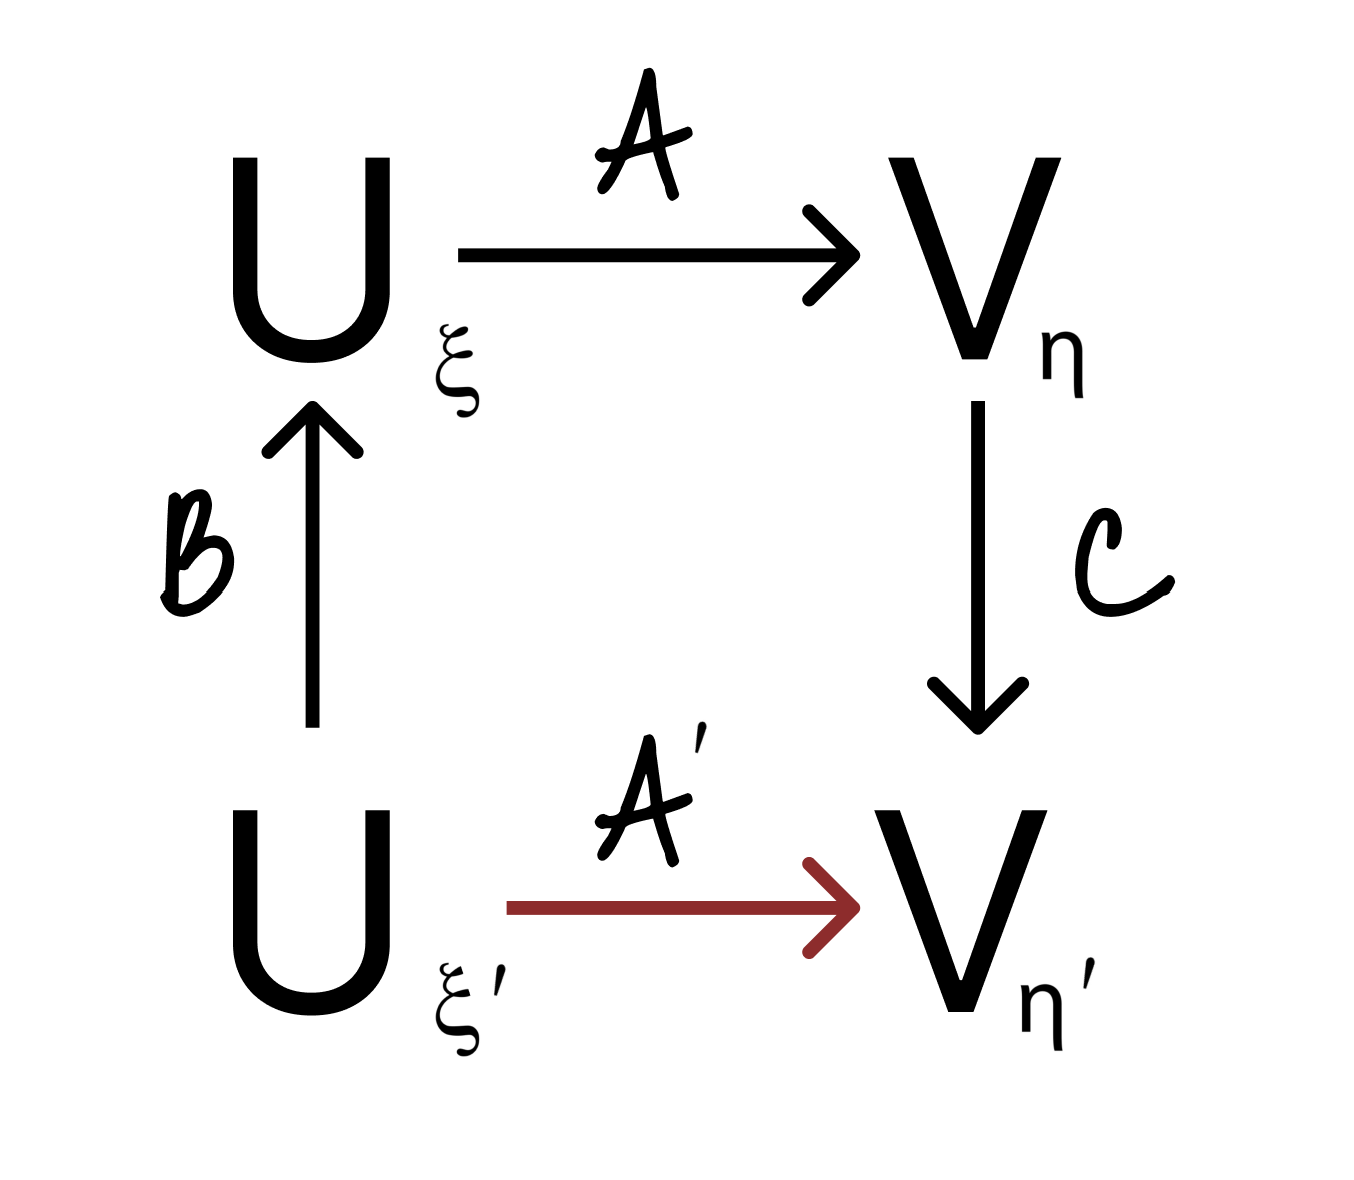
\includegraphics[width = 5cm]{assets/7_2_1.png}
\end{center}
    Воспользуемся данным рисунком, чтобы понять происходящее. Мы хотим найти матрицу $\mathcal{A}'$. Для этого, заметим, что преобразование $\mathcal{A}'$, это преобразование $\mathcal{B}$, потом примененное к нему преобразование $\mathcal{A}$, а после этого применненое к нему преобразование $\mathcal{C}$. То есть:
    $$\mathcal{A}'=\mathcal{C}\mathcal{A}\mathcal{B}$$

    Заметим, что матрица $\mathcal{B}$, это матрица перехода из $\xi$ в $\xi'$. Это так потому что у нас просто меняется базис (про саму матрицу перехода см. одноименный раздел). Матрица $\mathcal{C}$, это $T_{\eta' \rightarrow \eta}$. Откуда, исходя из двух утверждений сверху:
    $$A' = T_{\eta' \rightarrow \eta} A T_{\xi\rightarrow \xi'}\Rightarrow A' = T^{-1}_{\eta \rightarrow \eta'} A T_{\xi\rightarrow \xi'}$$ 

\hfill Q.E.D.
%todo

\deff{Следствие:} $A \in End(V)$. $e,e'$ базисы V. $A' = T^{-1}AT$, где $T = T_{e \to e'}$.

\deff{def:} квадратные матрицы $A$ и $B$ называются подобными, если $\exists$ невырожденная матрица $C$, такая, что: $B = C^{-1}AC$.

\textbf{Замечание:} матрицы линейного оператора в разных базисах подобны (см. следствие выше).

\subsection{Инварианты линейного отображения.}

\deff{Инвариатность} называется некоторое свойство объекта, которое не меняется при определенных действиях и преобразованиях.

$\mathcal{A}$ - линейное отображение. Ранг и дефект инварианты относительно выбора базиса.

Пусть $\mathcal{A} \in End(V)$. Пусть $e_1,\ldots, e_n$ базис $v$.

Как мы знаем, $\exists! D$ n-форма, такая что $D(e_1,\ldots e_n) = 1$. Тогда 
\deff{определитель} \deff{линейного оператора}:
$$\det \mathcal{A} := det(\mathcal{A}e_1,\ldots,\mathcal{A}e_n) = D(\mathcal{A}e_1,\ldots ,\mathcal{A}_n)$$ 
\textbf{Замечание:} $\det \mathcal{A} = D(\mathcal{A}e_1,\ldots ,\mathcal{A}_n) = D({A}e_1,\ldots ,{A}_n) = \det A$ --- определение определителя линейного оператора и матрицы соотносятся.

\thmm{Теорема:}

$\forall\mathcal{A}  \in End(V), \det \mathcal{A} = \det A$.

\textbf{Доказательство:}

Возьмем $e = (e_1,\ldots, e_n)$ базис $V$. Тогда:
$$\mathcal{A}  \xleftrightarrow{\text{вз. однозначно}} A = (a_{ij})_{n\times n}$$
$$\det \mathcal{A} = D(\mathcal{A}e_1,\ldots,  \mathcal{A} e_n)  = D(\sum\limits_{i=1}^na_{i1}e_{i_1},\ldots,\sum\limits_{i=1}^n a_{in}e_{i_n}) =$$$$\xLeftrightarrow{\text{тк $D$ - $n$ форма}}\det \mathcal{A}=\sum\limits_{i_1=1}^n\ldots \sum\limits_{i_n=1}^n a_{i_11}\cdot\ldots\cdot a_{i_nn} D(e_{i_1}\ldots,e_{i_n}) = $$
$$= \sum\limits_{\sigma \in S_n}  a_{i_11}\cdot\ldots\cdot a_{i_nn} \cdot (-1)^{\varepsilon(\sigma)}D(e_1,\ldots,e_n)=\det A$$

\hfill Q.E.D.

\textbf{Замечание:} $A$ и $B$ подобные матрицы, то $\det A = \det B$. 

\textbf{Замечание:} $\det \mathcal{A}$ \uline{инвариант} линейного оператора, он не зависит от базиса.

\textbf{Следствие 1:} $\forall n$ - форма $f$ на $V$:
$$\forall \xi_1,\ldots, \xi_n \in V: f(\mathcal{A}\xi_1.\ldots, \mathcal{A}\xi_n) =\det A f(\xi_1,\ldots, \xi_n)$$
\textbf{Доказательство:}

Возьмем $e = (e_1,\ldots,e_n)$ базис $V$. $\mathcal{A} \xleftrightarrow{e}A$. Это значит, что мы берем матрицу линейного оператора в данном базисе.
$$f(\mathcal{A}e_1.\ldots, \mathcal{A}e_n) \overset{\text{из доказательства теоремы}}{=}\det Af(e_1,\ldots,e_n)$$
На самом деле $\alpha = f(e_1.\ldots,e_n)$, поэтому:
$$\forall \xi_1,\ldots,\xi_n : g(\xi_1,\ldots,\xi_n):= f(\mathcal{A}\xi_1,\ldots, \mathcal{A} \xi_n)$$
Заметим, что $g$ - полилинейное, тк $f$ полилин. и $\mathcal{A}$ - лин. отобр. Также $g$ - антисим, тк $f$ - антисим. Откуда $g$ - $n$-форма. Заметим интересный факт:
$$g(e_1,\ldots,e_n) = f(\mathcal{A}e_1,\ldots,\mathcal{A}e_n) = \det A \cdot f(e_1,\ldots,e_n)$$
Откуда:
$$ g(\xi_1,\ldots,\xi_n)= g(e_1,\ldots,e_n) D(\xi_1,\ldots,\xi_n) = \det A  \cdot \alpha D(\xi_1,\ldots,\xi_n) = \det A \cdot f(\xi_1,\ldots,\xi_n)$$
\hfill Q.E.D.

\textbf{Замечание:} Мы можем вывести 9-ое свойство определителя по-другому. Пусть $\mathcal{A} = A_{n\times n}$ --- линейный оператор умножения.
$f = D$, $B_j \in K^n$. Тогда:
$$det(AB_1,\ldots, AB_N) = \det A \cdot \det B $$
\textbf{Следствие 2:}
$\mathcal{A},\mathcal{B} \in End(V) \Rightarrow \det(\mathcal{A} \mathcal{B}) = \det \mathcal{A} \cdot \det \mathcal{B}$

\textbf{Доказательство:}

Пусть $e$ - базис $V$. Тогда $\mathcal{A} \xleftrightarrow{e}A, \mathcal{B}\xleftrightarrow{e}B$. Также $\mathcal{A}\mathcal{B} \xleftrightarrow{e}AB$ по свойству. Откуда:
$$\det \mathcal{A}\mathcal{B} = \det(AB) = \det A \cdot \det B = \det \mathcal{A} \cdot \det\mathcal{B}$$
\hfill Q.E.D.

\textbf{Следствие 3:} $\mathcal{A} \in Aut(V) \Leftrightarrow \det A \neq 0$. Причем $\det \mathcal{A}^{-1} = \cfrac{1}{\det \mathcal{A}}$

\textbf{Доказательство:}
$$\mathcal{A} \in Aut(V) \Leftrightarrow \begin{cases}
    \mathcal{A} \in End(V) \\
    \text{изоморфизм}
\end{cases} \Leftrightarrow \begin{cases}
    \mathcal{A} \in End(V)\\
    def \mathcal{A} = \dim \ker \mathcal{A} = 0
\end{cases} \Leftrightarrow $$
$$\Leftrightarrow\begin{cases}
    \mathcal{A}\in End(V) \\
    rg \mathcal{A} = n
\end{cases} \Leftrightarrow \begin{cases}
    \mathcal{A} \xleftrightarrow{e} A,\det A \neq 0 \\
    \rg A = n
\end{cases}$$
Мы знаем, что существует $\mathcal{A}^{-1}$. А также $\mathcal{A}\cdot \mathcal{A}^{-1}=\varepsilon$. Откуда по свойству 3 получаем, что $\det\mathcal{A} ^{-1}=\det \mathcal{A}$.

\hfill Q.E.D.

\textbf{Следствие 4:} $\det( \mathcal{A} \mathcal{A}^{-1})= 1 = \det  \mathcal{A} \cdot \det \mathcal{A}^{-1}$


Вспомним старое определение $tr A = \sum\limits_{i=1}^n a_{ii}$ - \emph{след матрицы}.

\thmm{Теорема (о tr подобных матриц)}

Если $A$ и $B$ подобны, то $tr A = tr B$.

\textbf{Доказательство:}

$A$ и $B$ подобны $\Leftrightarrow\exists C :B =C^{-1}AC$. Пусть $C^{-1} = S = (s_{ij})$. Откуда:
$$tr B = \sum\limits_{i=1}^n b_{ii} = \sum\limits_{i=1}^n \sum\limits_{j=1}^ns_{ij} (AC)_{ji} = \sum\limits_{i=1}^n \sum\limits_{j=1}^n \sum\limits_{k=1}^n s_{ij}\cdot a_{jk} \cdot c_{ki} = \sum\limits_{j=1}^n\sum\limits_{k=1}^n a_{jk}\sum\limits_{i=1}^nc_{ki}s_{ij}$$
Заметим, что $(CS)_{kj} = \delta_{kj}$, где $\delta_{kj}=\begin{cases}
    1, k=j\\
    0, k\neq j
\end{cases}$. Так что получаем, что 
$$tr B = \sum\limits_{i=1}^n a_{ii} = tr A$$
\hfill Q.E.D.

\textbf{Следствие:} $\forall \mathcal{A} \in End(V) \Rightarrow tr(A) = tr A'$, где $A$ и $A'$ матрицы оператора $\mathcal{A}$ в базисе $e$ и $e'$ соответственно.

\deff{def:} $\mathcal{A} \in End(V), tr \mathcal{A} = tr A$ --- \deff{след оператора}.

\textbf{Замечание:} след оператора инвариантен из следствия выше.

\deff{def:} Линейное подпространство $L \subset V$ называется \deff{инвариантным} относительно линейного оператора $\mathcal{A}\in End(V)$, если $\forall v \in L, \mathcal{A} v \in L$.

\thmm{Теорема 1:}

$L \subset V$ - линейное подпространство. $L$ - инвариантно относительно $\mathcal{A} \in End(V)$. Тогда $ \exists $ базис пр-ва $V$ матрица, такой что матрица оператора $\mathcal{A}$ в этом базисе будет иметь \emph{ступенчатый вид}, при этом размерность $A^1 = k \times k,  \, k = \dim L$.
$$A =\begin{pmatrix}
    A^1 & *\\
    \zero & A^2
\end{pmatrix}$$
\textbf{Доказательство:}

$L = \span (e_1,\ldots, e_k)$ - базис $L$.

Дополним базис $L$ до базиса $V$: $V = \span (e_1,\ldots, e_k, e_{k+1},\ldots,e_n)$.

Запишем матрицу $A$ по определению:

$$\forall e_i\in L:\mathcal{A}e_i \in L  \Rightarrow \mathcal{A}e_i = \sum\limits_{j=1}^ka_{ji}e_j \leftrightarrow A_i = \begin{pmatrix}
    a_{1i}\\
    \vdots\\
    a_{ki}\\
    0\\
    \vdots\\0
\end{pmatrix}$$ 
Откуда $A = \begin{pmatrix}
    a_{11}&\ldots&a_{1k} & * & \ldots & *\\
    \vdots&\ddots & \vdots &\vdots& \vdots & \vdots\\
      a_{k1}&\ldots &  a_{k1} &\vdots& \vdots & \vdots\\
      0&\ldots &  0 &\vdots& \vdots & \vdots\\
        0&\ldots &  0 &*& \ldots & *\\
\end{pmatrix} \Rightarrow A^1 = \begin{pmatrix}
     a_{11}&\ldots&a_{1k}\\
     \vdots&\ddots & \vdots\\
     a_{k1}&\ldots &  a_{k1} \\
\end{pmatrix}$

\hfill Q.E.D.

\thmm{Теорема 2:}

$V = \bigoplus\limits_{i=1}^m L_i$, $L_i$ инвариантны отн. $\mathcal{A}$.
$\Rightarrow \exists$ базис пр-ва $V$, такое что м-ца оператора $\mathcal{A}$ будет иметь блочно-диагональный вид: 
$$
\begin{pmatrix}
    A^1 &\ldots&\ldots& \zero\\
    \vdots &A^2&\ldots& \vdots\\
    \vdots  & \vdots &\ddots& \vdots\\
    \zero & \ldots &\ldots& A^n
\end{pmatrix}$$
\textbf{Доказательство:}

Пусть базис $V \overset{\text{по эквив. условию $\oplus$}}= $ объединение базисов $L_i$.
$$L_i = \span(e_1^i,\ldots ,e_{k_i}^i),\dim L_i = k_i$$
Построим матрицу по определению. Не трудно заметить, что для каждого $L_i$ из доказательства прошлой теоремы, все кроме соотв. строчек для $L_i$ будет зануленно.

\hfill Q.E.D.

\textbf{Замечание:} $A_i \leftrightarrow A|_{L_i}\in End(L_i)$.


\thmm{Теорема 3.}

$V = \bigoplus\limits_{i=1}^m L_i$, $L_i$ инвариантны отн $\mathcal{A} \Rightarrow \Im\mathcal{A} = \bigoplus\limits_{i=1}^m  \Im \mathcal{A}|_{L_i}$, где
$\mathcal{A}|_{L_i}\in L(L_i,V)$


\textbf{Доказательство:}
$$V = \bigoplus\limits_{i=1}^mL_i \xLeftrightarrow{\text{из т. об экв. опр. прямой суммы}} \forall v \in V: \exists! v = \sum\limits_{i=1}^mv_i, v_i \in L_i$$
$$\forall  v \in V: \Im \mathcal{A}\ni\mathcal{A}v = \mathcal{A}\sum\limits_{i=1}^m v_i =\sum\limits_{i=1}^m\mathcal{A}v_i\in \Im A|_{L_i}$$
Тогда всё, что нам осталось проверить это то, что наши пространства дизъюнкты. Но, если присмотреться к тому, что у нас написано, то у нас для любого вектора из $\Im \mathcal{A}$ существует лишь одно разложение через $\Im A|_{L_i}$, что соответствует эквивалентному определению прямой суммы.

\hfill Q.E.D.
\subsection{Собственные числа и собственные векторы лин. оператора}

$\lambda \in K $ называется \deff{собственным числом} $\mathcal{A} \in End(V)$, если $\exists v \in V,v\neq 0$. $\mathcal{A} v = \lambda v$. Такой $v$  называют \deff{собственным вектором} собственного числа $\lambda$.

$$\lambda \in K: \begin{cases}
    \mathcal{A} v =\lambda v\\
    v\neq 0
\end{cases} \Leftrightarrow \begin{cases}
    (A-\lambda \varepsilon)v = 0 \\
    v \neq 0
\end{cases} \Leftrightarrow\begin{cases}
    v \in \ker (A-\lambda\varepsilon)\\
    v\neq 0
\end{cases}\Leftrightarrow $$

$\Leftrightarrow v$ собственный вектор собственного числа  $\lambda$.

$V_{\lambda} = \ker(A-\lambda\varepsilon) $ %написать это в 2 строчки
--- \deff{собственное подпространство} $\mathcal{A}$ соответств. с.ч. $\lambda$. Это  {мн-во всех с.в. $V$, отвечающим с.ч. $\lambda$  и нулевой вектор}.

$\gamma(\lambda) = \dim V_{\lambda}$ --- \deff{геометрическая кратность}.

\textbf{Свойства:}
\begin{enumerate}
    \item $V_{\lambda}$ инвариантно относительно $(\mathcal{A}-\lambda \varepsilon)$.
    \item $V_{\lambda}$ инвариантно относительно $\mathcal{A}$.
    \item $\gamma(\lambda)$ инвариант относительно базиса.
\end{enumerate}

\textbf{Условие существования с.ч.:} \\
$\lambda \in K_{\mathcal{A}}$ - с.ч., $v$ - с.в. $\Leftrightarrow \ker (A-\lambda\varepsilon)$ нетривиально $ \Leftrightarrow def(\mathcal{A} - \lambda\varepsilon) \ne 0 \Leftrightarrow rg(\mathcal{A} - \lambda\varepsilon) \ne n \Leftrightarrow \det(\mathcal{A} - \lambda \varepsilon) = 0$

Тк определитель линейного оператора  инвариантен, то:
$$\det(\mathcal{A} - \lambda \varepsilon) = 0 \Leftrightarrow \det({A} - \lambda E) = 0$$
\deff{def:} $\chi(t) = \det (\mathcal{A} - t\varepsilon)$ - \deff{характеристический многочлен} оператора $\mathcal{A}$.

Т.к. $\det$ оператора инвариантен $\chi(t) = \det (A - tE)$, где $A$ - матрица линейного оператора $\mathcal{A}$ в некотором базисе.
$$\chi(t) =\begin{vmatrix}
    a_{11} -t & a_{12} & \ldots & a_{1n} \\
    a_{21} & a_{22}-t & \ldots & \vdots\\
    \vdots & \vdots & \ddots & \vdots\\
    a_{n1} & a_{n2} & \ldots & a_{nn}-t
\end{vmatrix} = (-1)^{n}\cdot t^n + (-1)^{n-1}(tr At^{n-1}) + \ldots + \det A$$
По теореме Виета:
$\begin{cases}
t_1 +\ldots+t_n = tr A\\
t_1\cdot \ldots \cdot t_n = \det A
\end{cases}$
Заметим, что $\lambda$ с.ч. $\mathcal{A} \Leftrightarrow\begin{cases}
    \lambda \in K\\
    \chi(\lambda) = 0 \text{ - корень хар. мн.}
\end{cases}$

\textbf{Замечание.} Если все корни хар. мн. $\in K \Rightarrow$ $\begin{cases}
\lambda_1 +\ldots+\lambda_n = tr A\\
\lambda_1\cdot \ldots \cdot \lambda_n = \det A
\end{cases}$

\deff{def:} \deff{Спектром} оператора $\mathcal{A}$ называется множество $\{ (\lambda$, $\alpha(\lambda)) \}$, 
$\alpha(\lambda)$ - кратность $\lambda$ лин. оператора в хар. уравнении (\emph{алгебраическая кратность}). Спектр это множество пар.

\deff{def:} \deff{Простой спектр} --- все кратности -  единички.


\thmm{Теорема 1:}

$\forall \mathcal{A}\in End(V)$. $\forall \lambda$ с.ч. $\mathcal{A} : 1\leq \gamma(\lambda)\leq \alpha(\lambda)$

\textbf{Доказательство:}

$\lambda$ с.ч. $\mathcal{A} \Leftrightarrow \ker(\mathcal{A}-\lambda \varepsilon)= V_{\lambda}$ не тривиально $\Leftrightarrow \gamma_1=\dim V_\lambda\geq 1$.

Пусть $\dim V_{\lambda} = \gamma$, $V_{\lambda}$ инвариантно относительно $\mathcal{A} \Rightarrow$ по т-ме 1 об инв. подпр. существует $V$ такой, что матрица оператора $\mathcal{A}$ будет иметь ступенчатый вид:
$$A =\begin{pmatrix}
    A^1 & *\\
    \zero & A^2
\end{pmatrix}$$
$$\dim A^1 = \gamma \times \gamma,V = \span(e_1,\ldots, e_{\gamma},e_{\gamma+1},\ldots,e_{\gamma})$$

При построении матрицы оператора $\mathcal{A}$:

$\mathcal{A}e_i = \lambda e_i \leftrightarrow A_i = \begin{pmatrix}
    \vdots \\
    0\\
    \lambda\\0\\\vdots
\end{pmatrix}$ - $\lambda$ - на $i$-ой строчке. Немного распишем:

$$\chi(t) = \det(A-tE) =\begin{vmatrix}
    A^1-tE_{\gamma\times\gamma} & *\\
    \zero & A^2 -tE_{(n-\gamma)\times(n-\gamma))}
    \end{vmatrix} \overset{\text{по 6-ому св-ву опр}}=$$
    
    
    $$= |A^1-tE||A^2-tE|=\chi_{A^1}(t)\cdot \chi_{A^2}(t)=(\lambda-t)^\gamma\chi_{A_2}(t) \Rightarrow$$
    $ \Rightarrow \lambda $ корень $\chi(t)$, причем кратность $\geq \gamma$, т.к $\lambda$ может оказаться корнем $\chi_{A^2}$

\hfill Q.E.D.


\thmm{Теорема 2:}

$\lambda_1,\lambda_2,\ldots,\lambda_n$ попарно различные с.ч $\mathcal{A}$, $v_1,\ldots,v_n$ соответ. с.в.

$\Rightarrow v_1,\ldots,v_n$ --- лин. независимы.

\textbf{Доказательство:}

Докажем по индукции:

\textbf{База} $m = 1: \lambda_1,v_1 \Rightarrow$ лин. незав.

\textbf{ИП}: Пусть верно для $m$, докажем для $m+1$:

\uline{От противного:} Пусть $\lambda_1,\ldots,\lambda_m,\lambda_{m+1}$ попарно различные собственные числа. 

$v_1,\ldots,v_m$ - линейно независимы по ИП. $v_1,\ldots,v_m,v_{m+1}$ - линейно зависимы. Откуда: $v_{m+1}=\sum\limits_{i=1}^m \alpha_i v_i$. С одной стороны:
$$\mathcal{A} v_{m+1} = \lambda_{m+1} v_{m+1} = \lambda_{m+1}\sum\limits_{i=1}^m\alpha_iv_i$$
C другой стороны:
$$\mathcal{A} v_{m+1} =\mathcal{A}\sum\limits_{i=1}^m \alpha_i  v_i  =\sum\limits_{i=1}^m \alpha_i \mathcal{A} v_i = \sum\limits_{i=1}^m\alpha_i \lambda_i v_i$$
$$\sum\limits_{i=1}^m(\lambda_{m+1}-\lambda_i)a_i v_i = 0$$

% у меня в конспекте такое доказательство с лекции, которое показалось понятнее:
% все v_i не нули, все разности лямбд тоже не нули
% тогда все альфы нули, но тогда v_{m + 1} = 0, противоречие
Но мы знаем, что $v_1,\ldots,v_m$ линейно независимы. Откуда эта линейная комбинация тривиальна, но с другой стороны, она такой быть не может, потому что $\exists \alpha_i\neq 0$, для которого $v_i$ не равен нулю, а так же, исходя из того что искомые с.ч. попарно различны, то $v_{m+1}-v_i\neq 0$. Откуда комбинация нетривиальна. 

Противоречие.

\hfill Q.E.D.

\textbf{Следствие:} $\lambda_1, \ldots,\lambda_m$ попарно различные с.ч. $\mathcal{A} \Rightarrow \bigoplus\limits_{i=1}^m V_{\lambda_i}$, т.е $V_{\lambda_i}$ дизъюнктны.

\textbf{Доказательстсво:}
$$\zero = v_1 + \ldots+ v_m, v_i \in V_{\lambda_i}$$
Если в сумме какой-то из векторов не нулевой, то это собственный вектор, а собственные вектора для различных с.ч. линейно независимы. Противоречие. Откуда все вектора в сумме нулевые, откуда подпространства дизъюнктны.

\hfill Q.E.D.

\thmm{Теорема 3:}

$V = \bigoplus\limits_{i=1}^mL_i$, $L_i$ инвариантно относительно $\mathcal{A} \in End(V)$

$\Rightarrow \chi(t) = \det(\mathcal{A} - t\varepsilon) = \prod\limits_{i=1}^m\chi_{\mathcal{A}_i}(t) $.

\textbf{Доказательство:}

Смотрим теорему 3 об инв. подпр. Матрица A - блочно-диагональная:
$$A = \begin{pmatrix}
    A^1 &\ldots&\ldots& \zero\\
    \vdots &A^2&\ldots& \vdots\\
    \vdots  & \vdots &\ddots& \vdots\\
    \zero & \ldots &\ldots& A^n
\end{pmatrix}$$
  Тогда $\chi(t) = \det(A-tE) \overset{\text{по 6-ому свойству опр.}}= \prod\limits_{i=1}^m \det(A^i-tE) = \prod\limits_{i=1}^m \chi_{A_i}(t) $

\hfill Q.E.D.


\subsection{Оператор простой структуры (о.п.с). Проекторы. Спектральное разложение. Функция от диагонализированной матрицы.}

$\mathcal{A} \in End(V)$ называется \deff{оператором простой структуры} (о.п.с), если $\exists$ базис пространства $V$ такой, что матрица оператора $\mathcal{A}$ в этом базисе имеет диаг. вид.
$$\Lambda = diag(\lambda_1,\ldots,\lambda_n)=\begin{pmatrix}
    \lambda_1 & \ldots & 0 \\
    \vdots & \ddots & \vdots\\
    0 & \ldots &\lambda_n
\end{pmatrix}$$

Заметим, что в таком случае  собственные числа  оператора $\mathcal{A}$ будут $\lambda_i$, а так же собственные вектора этих чисел - соотв. столбики (легко проверить умножением). Отсюда  все корни характ. многочлена  $\chi \in K \Leftrightarrow \sum\limits_{\lambda \text{-с.ч.} \mathcal{A}}\alpha(\lambda) = n = \dim V$.



\thmm{Теорема:}

$\forall A \in End(V)$, если  $\sum\limits_{\lambda \text{-с.ч.} \mathcal{A}} \alpha(\lambda)= n$, то тогда:
$$\mathcal{A} \text{ - о.п.с} \Leftrightarrow \forall\lambda \text{ - с.ч }: \gamma(\lambda) = \alpha(\lambda) \Leftrightarrow \sum\limits_{\lambda \text{-с.ч.} \mathcal{A}}\gamma(\lambda) = n = \dim V$$
\textbf{Доказательство:}

$ \sum\limits_{\lambda \text{-с.ч.} \mathcal{A}} \alpha(n) = n \Leftrightarrow$ все корни $\chi \in K$, откуда $\mathcal{A}$ -  о.п.с.

$\mathcal{A}$ о.п.с. $\Leftrightarrow \exists$ базис $V$ такой, что матрица диагональна $\Leftrightarrow$ $$\Leftrightarrow V = \bigoplus\limits_{\lambda - \text{с.ч.}}V_{\lambda} \Leftrightarrow \sum\limits_{\lambda - \text{с.ч.}}\gamma(\lambda) = n =\dim V$$
\hfill Q.E.D.

\textbf{Следствие.} Если все корни характ. многочлена $\in K$, а также все $\alpha(\lambda)=1$ (спектр простой), то $\mathcal{A}$ - о.п.с.

\deff{def:} $A_{n\times n}$ называется \deff{диагонализируемой}, если  она подобна диагональной.

\thmm{Теорема (критерий диагональности матрицы $A$)}

\sout{это перепишетмя}

$A$ подобна диагональной $\Leftrightarrow$ матрица о.п.с $\mathcal{A}$ в нек. базисе

\textbf{Доказательство:}

\begin{itemize}
    \item  \fbox{\(\Rightarrow\)}
    
    Пусть $A$ - диагонализируемая $\Leftrightarrow$ подобна диагональной $\Leftrightarrow$ $\exists$ невырожд T: $T^{-1}AT=\Lambda=diag(\lambda_1,\ldots,\lambda_n)$. $V$ - линейное пространство над полем $K$. $e = (e_1,\ldots,e_n)$ - базис V.

    Пусть $A$ - матрица в базисе $e$. Тогда $Ae_j = \sum\limits_{i=1}^n=a_{ij}e_i$.$v =(v_1,\ldots,v_n)$ - базис.\\Откуда $v_1,\ldots,v_n = (e_1,\ldots,e_n)T_{e\rightarrow v} \Rightarrow \mathcal{A}\xleftrightarrow{v} A' = T^{-1}AT=\Lambda$ 
    \item \fbox{\(\Leftarrow\)}
    $\mathcal{A}$ о.п.с, $A$ - матрица в некотором базисе $e= (e_1,\ldots,e_n)$.
    Возьму $v_1, ..., v_n$ - базис V, где $v_i$ - собственный вектор $\mathcal{A}$. Заметим, что так как $\mathcal{A}$ о.п.с, то такой базис существует

   Теперь давайте возьмем матрицу перехода из $T_{e\rightarrow v}$. Тогда $\mathcal{A}\xleftrightarrow{v} A' = T^{-1}AT=\Lambda \Rightarrow A$ подобна диагональной   

    \hfill Q.E.D.
\end{itemize}
   
\textbf{Алгоритм поиска диагонального представления матрицы подобной диагональной:}
\begin{enumerate}
    \item найти спектр: если все корни $\chi \in K $, переходим к п2.
    \item найти все $\gamma(\lambda)$, если $\forall \lambda$ с.ч $\gamma(\lambda) = \alpha(\lambda)$, то перейти к п3.
    \item $T_{\text{кан.}\rightarrow v} = (v_1,\ldots,v_n)$ $T^{-1}AT = \Lambda$
\end{enumerate}